% !TeX program = pdflatex

\documentclass[]{article}

% Packages
\usepackage{graphicx}
\usepackage{biblatex}
\usepackage{subfiles}
\usepackage{standalone}
\usepackage{import}
\usepackage{amsmath}
\usepackage{amssymb} % For math symbol E (expected)
\usepackage{datetime} % Title page current date
\usepackage{hyperref} % For now I'm just seeing the green bounding boxes around citations
\usepackage{url} % For URL references

% For figures
\usepackage{tikz}
\usetikzlibrary{shapes,arrows,positioning,automata,calc}


% References
\addbibresource{references.bib}




\begin{document}

% Cover (Title page)
\begin{titlepage}
    \begin{center}
        \vspace*{1cm}
        
        
\includegraphics[width=0.2\textwidth]{images/ou_logo.png}\\
        The Open University of Israel\\
        Department of Mathematics and Computer Science
        
        \vspace{2cm}
        
        {\Large \textbf{An Overview of Deep Learning Techniques for Image and Video Generation}}
        \vspace{1.5cm}
        
        Final paper submitted as partial fulfillment of the requirements\\towards an M.Sc. degree in Computer Science\\
        The Open University of Israel\\
        Department of Mathematics and Computer Science
        
        \vspace{1cm}
        
        By \\
        \textbf{Shlomi Domnenko}
        
        \vspace{1cm}
        
        Prepared under the supervision of \textbf{Dr. Mireille Avigal}
        
        \vfill
        
        \textbf{May 2025}
    \end{center}
\end{titlepage}

% Table of Contents (ToC)
\tableofcontents
\newpage

% Abstract
\section{Abstract}

% TODO: Need to add more examples of good models, in particular video generation.

This research paper examines recent progress in image and video synthesis using machine learning (ML). While image synthesis has reached a considerable degree of maturity with the development of sophisticated deep learning models, video synthesis continues to present significant research challenges.

Deep generative models, particularly prominent models like DALL-E \cite{dalle}, Sora \cite{sora_website}, Midjourney \cite{midjourney-website}, have gained significant attention due to their ability to produce high-resolution and creative images and videos. In this paper we will focus on 3 image synthesis models and 3 video synthesis models that had a significant contribution to the advancement of the domain. In image synthesis will focus on VQ-GAN \cite{vqgan}, Stable Diffusion \cite{stable_diffusion} and Imagen \cite{imagen}. In video synthesis we will focus on Video-LDM \cite{video_ldm}, Stable Video Diffusion (SVD) \cite{stable_video_diffusion} and Make-a-Video \cite{make_a_video}.

This paper surveys the recent advancements in ML techniques for image and video generation. We explore the fundamental concepts underlying these techniques, focusing on how they learn to create realistic and compelling visual content. We place particular emphasis on the video generation domain, recognizing its immense potential and future applications.

% TODO: Add examples of models to "Diffusion Models", add references to mentioned models
The paper delves into various image generation models, including Variational Autoencoders (VAEs) \cite{vae}, Generative Adversarial Networks (GANs) \cite{gan}, and Diffusion Models (DMs) \cite{dpms}. We discuss their working principles, strengths, and limitations. Additionally, we explore the use of conditioning to control the output, temporal and spatial cohesion in video synthesis, dataset preparation and learning optimization. Finally, we explore video synthesis techniques that build upon these image generation models, highlighting their unique challenges and interesting points.
\newpage

% Introduction
\section{Introduction}

The field of image and video synthesis is large and continuously expanding. While image generation has come a long way, recent advancements in video synthesis emerged recently, highlighted by the significant breakthrough of OpenAI's Sora model \cite{sora_website}. A solid foundation in image synthesis techniques is essential to fully comprehend the methodologies and techniques involved in video synthesis.

In this work we will review two main models that are used as a basis in image and video generation models: Generative Adversarial Networks (GANs) \cite{gan} \ref{sec:gan} and Diffusion Probabilistic Models (DPMs) \cite{diffusion_models} \cite{ddpm} \ref{sec:ddpm}.

In generative models we are given a set of data points (e.g. images) and our goal is to create a new sample (new image) from this dataset. That is, we don't want to randomly select an image from the dataset, but rather we want to create a new image that does not appear in the dataset, but is similar to it. The key word is "similar" - mathematically speaking, we are talking about predicting the probability function of the dataset. That is, the model needs to learn the underlying distribution of the dataset and create new samples that represent the same distribution. Generative models provide an efficient method for analyzing and understanding unlabeled data in unsupervised learning.

Advanced image synthesis models like DALL-E \cite{dalle} and Stable Diffusion \cite{stable_diffusion} represent a significant milestone in the field. While recent models may not offer groundbreaking advancements, the landscape of long video synthesis remains relatively unexplored. Video synthesis presents unique challenges compared to image synthesis, primarily due to the introduction of the temporal dimension.

New models for generating images and videos are developed by building upon existing models, enhancing them through innovative techniques and adjustments. In this work we explore the VQ-GAN model \cite{vqgan} \ref{vqgan} which combines the GAN model \cite{gan} \ref{sec:gan} with the VQ-VAE model \cite{vqvae} \ref{vqvae} and the Transformer model \cite{transformer} (appendix \ref{appendix:transformers}) together. Notably, VQ-GAN generates images based on textual descriptions, converting text inputs into visual outputs that reflect the text's description. The VQ-VAE model, derived from the VAE model \cite{vae} \ref{sec:vae} and employing vector quantization technique \cite{vqvae} \ref{sec:vq}, is itself an advancement of the Autoencoder model \cite{autoencoder} \ref{sec:vae}. In short, understanding these models and their inner workings requires prior familiarity with their foundations and previous works.

Another example is the Variational Autoencoder (VAE) \cite{vae} \ref{sec:vae} model, which is used as a basis in VQ-VAE model. 

\begin{figure}[H]
    \centering
    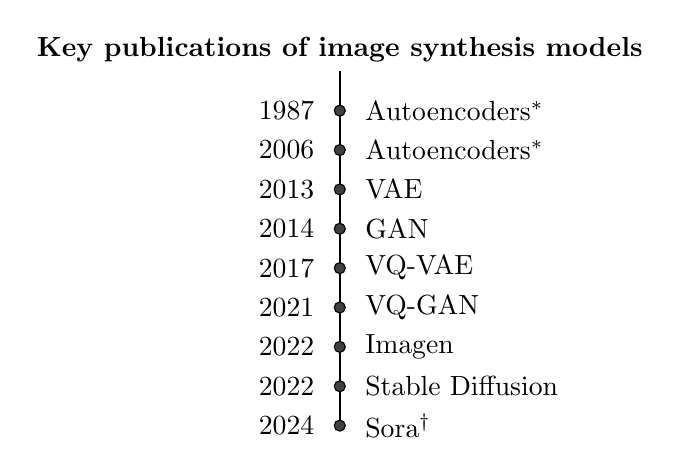
\begin{tikzpicture}
        \def\step{0.5} % step size for vertical spacing
        \def\numtimeline{9} % Number of events in the timeline

        % Define timeline line
        \draw[thick, color=black] (0,0) -- (0,-\numtimeline*\step);

        % Define timeline events with adjusted positions
        \foreach \i/\year/\text in 
        {
            1/1987/Autoencoders$^*$, 
            2/2006/Autoencoders$^*$, 
            3/2013/VAE, 
            4/2014/GAN, 
            5/2017/VQ-VAE,
            6/2021/VQ-GAN,
            7/2022/Imagen,
            8/2022/Stable Diffusion,
            9/2024/Sora$^\dag$
        } {
        \draw[fill=darkgray] (0,-\i*\step) circle (2pt);
        \node[anchor=east] at (-0.2,-\i*\step) {\year};
        \node[anchor=west] at (0.2,-\i*\step) {\text};
        }

        % Define timeline title
        \node[anchor=south] at (0,0) {\textbf{Key publications of image synthesis models}};
    \end{tikzpicture}
    \caption{Chronology of key image generation models publications $^*$The earliest mention of autoencoders appears in an 1986 publication \cite{autoencoder_original_paper_1986}, however the model was not widely used until 2006 when Hinton published a paper that uses autoencoders for dimensionality reduction \cite{autoencoder_2006_paper} which sparked interest in the model again.$^\dag$Although Sora \cite{sora_website} is not specifically an image generation model, it is considered a significant advancement in video synthesis field, which largely relies on image generation.}
    \label{fig:timeline}
  \end{figure}

\subsection{Mathematical Formulation of Generative Models}
Mathematically speaking, let $x$ be a random variable representing a single data point (e.g. an image) of a dataset ${x_1,x_2,...,x_n}$. And let $p(x)$ denote the true probability density function (PDF) of the dataset. Then our objective (as in generative modeling) is to learn a function $q(x;\theta)$ that approximates the true data distribution $p(x)$ (where $\theta$ is the model's parameters). The goal is to estimate $p(x)$ such that new samples $\hat{x} \in p(x)$ drawn from this distribution resemble the dataset.

Most of the time, it is infeasible to calculate directly $p(x)$ because computing the exact probability density for high-dimensional data is computationally expensive and often requires integrating over a large number of variables. This complexity leads to intractable calculations, making it difficult to directly model $p(x)$. Instead, we use various techniques to approximate it, and we denote it as: $q(x;\theta) \sim p(x)$.

\subsection{Approximating the Data Distribution}

In order to approximate $p(x)$ we can use a generative model, where the training objective is to learn the parameters $\theta$ of the model. The success or failure of the model to correctly approximate the dataset distribution can be evaluated using different loss functions, such as maximizing likelihood functions (Appendix \ref{appendix:likelihood_function}), minimizing Kullback-Leibler (KL) divergence, or using adversarial training loss (in the case of GANs).

\subsection{Sampling}

Once trained, the generative model can be used to generate new samples $\hat{x} \sim q(x;\theta)$. Sampling data point $\hat{x}$ will be consistent with the patterns and characteristics of the original dataset, as the model has learned to approximate the true data distribution. Each model will have different strategies to sample. For example, in GANs a random noise vector is sampled from a normal distribution and passed through the generator to generate a new sample, and in VQ-GAN a transformer is used to generate latent codes that are then passed through the decoder to generate an image.

\subsection{Evaluation metrics}

Evaluation of the trained model is done using metrics such as sample quality, diversity (variety in generated samples), and coverage (how well the model covers the data distribution). As we will find later, one of the main problems of the GAN model is called 'mode collapse' \ref{gan_mode_collapse} which causes instability of the model during training, which is manifested in large fluctuations in the loss function or in the fact that the generator fails to converge to an optimal solution that represents the entire distribution of training data. In other words, the model's output isn't diverse enough and only focuses on specific modes of the data distribution (e.g. generating only one type of image, like a cat, whereas the dataset is a collection of all animals).





\textbf{Inception Score.} One of the most common metrics used to evaluate the quality of generated samples is the Inception Score (IS) \cite{is_score}. The IS metric measures the quality and diversity of the generated samples. A good generative model should not only produce images that look visually realistic but also capture the underlying statistical properties of the dataset. A high IS score indicates that the generated samples are both realistic and diverse. IS uses pre-trained Inception V3 model \cite{inception_v3_model} to extract features and classify images to labels. The Inception V3 model is made of multiple convolutional layers and pooling layers and the last layers are fully connected layers with softmax activation function (output is probability of labels) that output the class labels (1000 classes). Two generative models are compared to each other with IS by running the same Inception V3 model, and comparing their scores relatively. The IS is calculated by first computing the conditional entropy of the generated samples given the class label: 

\[
    p(y) = \frac{1}{N} \sum_{i=1}^{N} p(y|x_i)
\] 

(where $y$ is the class label and $x$ is an image, $p(y|x)$ is the conditional probability of the label $y$ given image $x$) (i.e., the diversity of generated samples) and then computing the \textbf{KL divergence} between the marginal distribution of the generated samples and the conditional distribution:

\[
    D_{\text{KL}}(p(y|x) \| p(y)) = \sum_{y} p(y|x) \log \frac{p(y|x)}{p(y)}
\]

(where $p(y)$ is the marginal probability of the label across the set of generated images, and $D_{KL}$ is the Kullback-Leibler (KL) divergence between the conditional label distribution $p(y|x)$ and marginal label distribution $p(y)$). Finally, we get the IS score as:

\[
    \text{IS} = \exp \left( \frac{1}{N} \sum_{i=1}^{N} D_{\text{KL}}(p(y|x_i) \| p(y)) \right) = \exp(\mathbb{E}_{x \sim p_g} \left[ D_{\text{KL}} \left( p(y | x) \Vert p(y) \right) \right])
\]

Where $p_g$ is the distribution of the generated images. The IS score is the exponential of the sum of these two terms. A high IS score indicate that the generated samples are both realistic and diverse because $p(y|x)$ should be sharp (i.e. indicating generated samples are high quality), and $p(y)$ should be uniform (i.e. generated samples are diverse).






\textbf{FID Score.} Frechet Inception Distance (FID) score \cite{fid_score} is an improvement on the Inception Score and is more recent. The FID score also measures the similarity between the generated samples and the real data distribution, and the diversity. FID aims to capture this by comparing the feature distributions, not just individual image similarity. The lower the FID score, the better the model is at generating samples that resemble the real data distribution. FID leverages a pre-trained image classification model (which is also typically Inception V3 model), to extract high-level features from both the generated images and the dataset. These features capture the essential characteristics of the images, like shapes, textures, and object relationships. Then, its possible to compare generative models based on the similarity of these features relatively to the same dataset, compared to just looking at the labels in Inception Score. The FID score is calculated as:

\begin{equation}
    \text{FID} = ||\mu_x - \mu_g||^2 + Tr(\Sigma_x + \Sigma_g - 2(\Sigma_x\Sigma_g)^{1/2})
    \label{eq:fid_score}
\end{equation}

where $\mu_x$ and $\Sigma_x$ are the mean and covariance of the feature distribution of the dataset, and $\mu_g$ and $\Sigma_g$ are the mean and covariance of the feature distribution of the generated images. The FID score is the Euclidean distance between the means and the trace (matrix operation) of the covariance matrices. A lower FID score indicates that the generated samples are more similar to the real data distribution.


\newpage

% VAE
\section{Variational Autoencoder}
\label{sec:vae}

Variational Autoencoder (VAE) \cite{vae} is generative model is used to learn the underlying distribution of data and generate new samples (similar to the dataset). The model consists of 3 main components: an encoder, latent space (sometimes called 'code vectors' or 'bottleneck layer') and a decoder. The main idea behind VAE is to use the autoencoder model \cite{autoencoder} \cite{autoencoder2} to compress large dimensional vectors (in our case, images) into smaller, low dimension vectors that represent the underlying features hidden within the input data. These code vectors are then fed into a decoder network which reconstructs the image (i.e. high dimensional vector).


\begin{figure}[h]
    \centering
    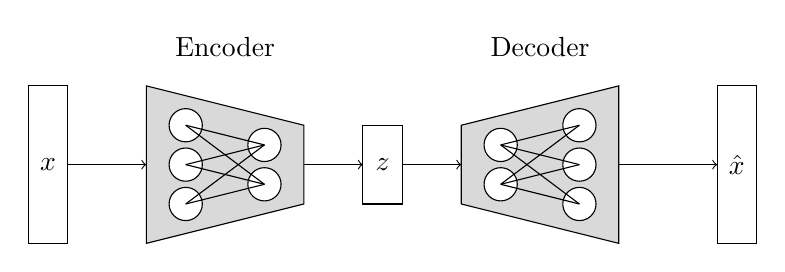
\begin{tikzpicture}
        % Center point of encoder
        \coordinate (E_CENTER) at (1, 1);
        \coordinate (INPUT_TEXT) at (-0.25, 0.5);



        % Draw input vector
        \draw ($(INPUT_TEXT) + (-0.25, -0.5)$) rectangle ($(INPUT_TEXT) + (0.25, 1.5)$) node[pos=.5] {$x$};
        \draw[->] ($(E_CENTER) + (-1, 0)$) -- (E_CENTER);

        








        % Draw the encoder
        \node at ($(E_CENTER) + (1, 1.5)$) {Encoder};
        
        \coordinate (A) at ($(E_CENTER) + (0, -1)$);
        \coordinate (B) at ($(E_CENTER) + (2, -0.5)$);
        \coordinate (C) at ($(E_CENTER) + (2, 0.5)$);
        \coordinate (D) at ($(E_CENTER) + (0, 1)$);
        \draw[fill=gray!30] (A) -- (B) -- (C) -- (D) -- cycle;
        
        % Define the coordinates for the first set of circles (3 neurons)
        \coordinate (n1) at ($(E_CENTER) + (0.5, -0.5)$);
        \coordinate (n2) at ($(E_CENTER) + (0.5, 0)$);
        \coordinate (n3) at ($(E_CENTER) + (0.5, 0.5)$);
        
        % Define the coordinates for the second set of circles (2 neurons)
        \coordinate (m1) at ($(E_CENTER) + (1.5, 0.25)$);
        \coordinate (m2) at ($(E_CENTER) + (1.5, -0.25)$);
        
        % Draw the first set of circles
        \foreach \i in {n1, n2, n3} {
            \filldraw[fill=white] (\i) circle (6pt);
        }
        
        % Draw the second set of circles
        \foreach \i in {m1, m2} {
            \filldraw[fill=white] (\i) circle (6pt);
        }
        
        % Draw arrows from each circle in the first set to each circle in the second set
        \foreach \i in {n1, n2, n3} {
            \foreach \j in {m1, m2} {
                \draw[-] (\i) -- (\j);
            }
        }






        % Draw code vector

        % Arrow in
        \coordinate (Z_TEXT) at ($(E_CENTER) + (3, 0)$);
        \draw[->] ($(E_CENTER) + (2, 0)$) -- ($(Z_TEXT) + (-0.25, 0)$);

        \draw ($(Z_TEXT) + (-0.25, -0.5)$) rectangle ($(Z_TEXT) + (0.25, 0.5)$) node[pos=.5] {$z$};
        
        % Arrow out
        \coordinate (D_CENTER) at ($(E_CENTER) + (4, 0)$);
        \draw[->] ($(Z_TEXT) + (0.25, 0)$) -- (D_CENTER);











        % Draw decoder
        \node at ($(D_CENTER) + (1, 1.5)$) {Decoder};
        
        \coordinate (A2) at ($(D_CENTER) + (0, 0.5)$);
        \coordinate (B2) at ($(D_CENTER) + (2, 1)$);
        \coordinate (C2) at ($(D_CENTER) + (2, -1)$);
        \coordinate (D2) at ($(D_CENTER) + (0, -0.5)$);
        \draw[fill=gray!30] (A2) -- (B2) -- (C2) -- (D2) -- cycle;
        
        % Define the coordinates for the first set of circles (2 neurons)
        \coordinate (n2_1) at ($(D_CENTER) + (0.5, 0.25)$);
        \coordinate (n2_2) at ($(D_CENTER) + (0.5, -0.25)$);
        
        % Define the coordinates for the second set of circles (3 neurons)
        % \coordinate (m2_1) at (1.5, 0.5);
        % \coordinate (m2_2) at (1.5, 1);
        % \coordinate (m2_3) at (1.5, 1.5);
        \coordinate (m2_1) at ($(n2_1) + (1, 0.25)$);
        \coordinate (m2_2) at ($(n2_1) + (1, -0.25)$);
        \coordinate (m2_3) at ($(n2_1) + (1, -0.75)$);
        
        % Draw the first set of circles
        \foreach \i in {n2_1, n2_2} {
            \filldraw[fill=white] (\i) circle (6pt);
        }
        
        % Draw the second set of circles
        \foreach \i in {m2_1, m2_2, m2_3} {
            \filldraw[fill=white] (\i) circle (6pt);
        }
        
        % Draw arrows from each circle in the first set to each circle in the second set
        \foreach \i in {n2_1, n2_2} {
            \foreach \j in {m2_1, m2_2, m2_3} {
                \draw[-] (\i) -- (\j);
            }
        }


        \coordinate (D_END) at ($(D_CENTER) + (2, 0)$);




        % Draw output vector
        \coordinate (X_OUT_TEXT) at ($(m2_2) + (2, 0)$);
        \draw[->] (D_END) -- ($(X_OUT_TEXT) + (-0.25, 0)$);
        
        \draw ($(X_OUT_TEXT) + (-0.25, -1)$) rectangle ($(X_OUT_TEXT) + (0.25, 1)$) node[pos=.5] {$\hat{x}$};
        
        % \node at (X_OUT_TEXT) {$\hat{x}$};
        
    \end{tikzpicture}
    \caption{Autoencoder architecture.}
\end{figure}


More formally, the encoder network takes an input data point $x$ and maps it to a latent space representation $z$, which is compressed representation of $x$. The input is a vector, therefor an image must be flattened from 2D to 1D vector. This flattening will become an issue later in image generation, as this action removes important spatial information and hidden structures in the image. Because of this, modifications were made to the VAE model which allows the capture of spatial information by using a CNN (Convolutional Neural Network) \cite{cnn} layers \cite{vae_cnn_example}, max pooling layers, and more. After compression, the latent vector $z$ is then passed onto the decoder for reconstruction. 

The reconstruction is learned by a reconstruction loss function, usually mean squared error (MSE) loss function:

\begin{equation}
    \text{MSE} = \frac{1}{N} \sum_{i=1}^{N} (y_i - \hat{y}_i)^2
\label{eq:mse}
\end{equation}

The MSE loss is common in image generation models, because this loss is used to ensure that the generated images closely resemble the original input images by comparing the distance between pixels (input image, output image). This objective motivates the model to reconstruct the image from latent vector to resemble the original image. However, this loss is not used alone usually, but in combination with more complex loss functions, as we will see later in VAE.

The code vectors learned by autoencoders, however, are one-to-one map of the input and code vector (deterministic mapping from input to code vectors). The model doesn't capture any semantic relationships between the data (e.g the code vectors of images of cats are scattered throughout the entire latent space, whereas in VAE, they are clustered together). The latent space in autoencoders is irregular and discontinuous, meaning a small change in the latent vector can lead to large unpredictable changes in the output. This makes interpolation in the latent space difficult. Variational autonecoder solve this problem. VAE regularizes the latent space by enforcing a prior distribution. This regularization leads to a smooth and continuous latent space (see figure \ref{fig:ae_vs_vae}), which allows the model to interpolate between the latent space smoothly, thus creating similar new images with different variations. VAEs also provide an explicit model of the data distribution by maximizing a variational lower bound on the likelihood of the data. In other words, VAE is probabilistic model instead of discrete mapper (like the autoencoder model).

\begin{figure}[h]
    \centering
    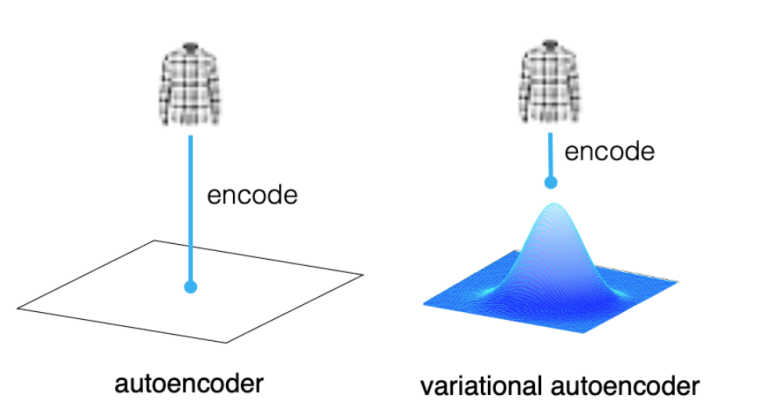
\includegraphics[scale=0.5]{images/autoencoder-vs-variational-autoencoder-point-vs-distribution-768x409.png}
    \caption{Illustration of mapping an input image to code vector (left) and mapping an input image to a distribution (right) \cite{ae_vs_vae}.}
    \label{fig:ae_vs_vae}
\end{figure}

At the heart of VAE lies the concept of latent variables (Appendix \ref{appendix:latent_variables}). Latent variables are hidden, unobserved variables that the model infers from the observed data (dataset). Latent variable models, such as VAE, take indirect approach to describing a probability distribution $p(x)$ over multi-dimensional variable $x$. Instead of directly writing the expression for $p(x)$, they model a joint distribution $p(x|z)$ of the data $x$ and an unobserved hidden latent variable $z$.

The variational aspect of VAE refers to the use of variational inference (VI) (Appendix \ref{appendix:variational_inference}). VI is used to used to approximate complex posterior distributions: 

\begin{equation}
p(z|x) = \frac{p(x|z) \cdot p(z)}{\int p(x|z) \cdot p(z) dz}
\label{eq:posterior}
\end{equation}

by transforming the problem into optimization problem. The denominator in eq. \ref{eq:posterior} is intractable because it involves integrating over all possible values of $z$, and $z$ is often relatively high-dimensional and its infeasible to evaluate exactly. Which is why VI is used, which approximates the true posterior distribution $p(z|x)$ with simpler, tractable distribution $q_\phi (z|x)$, parameterized by $\phi$.

The original VAE model uses fully connected layers at the encoder and decoder networks. However, in the image synthesis field, CNN layers (appendix \ref{appendix:cnn}) are used instead which are computationally less expensive and better capture the spatial information, for instance, its used in VQ-VAE (section \ref{sec:vqvae}) and PixelCNN \cite{pixelcnn}.

To generate an image, we first sample a latent variable $z$ from prior distribution $p(z)$, which is typically standard normal distribution $\mathcal{N}(0, 1)$. Then $z$ is passed to the decoder an an image $x$ is generated from the conditional distribution $p_\theta (x|z)$. 

\subsection{The Reparameterization Trick}
To enable backpropagation through the sampling process, VAEs use the reparameterization trick. This trick involves expressing the sampled latent variables $z$ as a deterministic function of the encoder's output and some random noise. Without this technique, backpropagation would not be possible through the sampling operation. The reason is that sampling is a non-differentiable operation, because sampling from a distribution involves randomness that does not have a gradient, and the gradients cannot be computed with respect to the parameters of the encoder. To make the sampling operation differentiable and thus allow gradients to flow through the network, the reparameterization trick is used. 

Specifically, if $\mu$ and $\sigma$ are the mean and standard deviation vectors outputted by the encoder, we can write:

\begin{equation}
    z = \mu + \sigma \cdot \epsilon
\end{equation}

where $\epsilon \sim \mathcal{N}(0, 1)$ is a standard normal random variable. This $\epsilon$ will not change throughout the training reigime. It is sampled once and fixed in place. This trick allows us instead of having full stochastic node that blocks flow of gradients, to having two parts: one where we can do backpropagation, and another part which is still stochastic but which we don't want to train because its fixed.


\begin{figure}[h]
    \centering
    \begin{tikzpicture}
        % Center point of encoder
        \coordinate (E_CENTER) at (1, 1);
        \coordinate (INPUT_TEXT) at (-0.25, 0.5);



        % Draw input vector
        \draw ($(INPUT_TEXT) + (-0.25, -0.5)$) rectangle ($(INPUT_TEXT) + (0.25, 1.5)$) node[pos=.5] {$x$};
        \draw[->] ($(E_CENTER) + (-1, 0)$) -- (E_CENTER);

        








        % Draw the encoder
        \node at ($(E_CENTER) + (1, 1.5)$) {Encoder $q_\phi(z|x)$};
        
        \coordinate (A) at ($(E_CENTER) + (0, -1)$);
        \coordinate (B) at ($(E_CENTER) + (2, -0.5)$);
        \coordinate (C) at ($(E_CENTER) + (2, 0.5)$);
        \coordinate (D) at ($(E_CENTER) + (0, 1)$);
        \draw[fill=gray!30] (A) -- (B) -- (C) -- (D) -- cycle;
        
        % Define the coordinates for the first set of circles (3 neurons)
        \coordinate (n1) at ($(E_CENTER) + (0.5, -0.5)$);
        \coordinate (n2) at ($(E_CENTER) + (0.5, 0)$);
        \coordinate (n3) at ($(E_CENTER) + (0.5, 0.5)$);
        
        % Define the coordinates for the second set of circles (2 neurons)
        \coordinate (m1) at ($(E_CENTER) + (1.5, 0.25)$);
        \coordinate (m2) at ($(E_CENTER) + (1.5, -0.25)$);
        
        % Draw the first set of circles
        \foreach \i in {n1, n2, n3} {
            \filldraw[fill=white] (\i) circle (6pt);
        }
        
        % Draw the second set of circles
        \foreach \i in {m1, m2} {
            \filldraw[fill=white] (\i) circle (6pt);
        }
        
        % Draw arrows from each circle in the first set to each circle in the second set
        \foreach \i in {n1, n2, n3} {
            \foreach \j in {m1, m2} {
                \draw[-] (\i) -- (\j);
            }
        }






        % Draw middle
        \coordinate (Z_TEXT) at ($(E_CENTER) + (3, 0)$);

        \coordinate (MIDDLE_BEGIN) at ($(Z_TEXT) + (-0.5, 0)$);
        \coordinate (MU_BEGIN) at ($(MIDDLE_BEGIN) + (0.25, 0.5)$);
        \coordinate (SIGMA_BEGIN) at ($(MIDDLE_BEGIN) + (0.25, -0.5)$);
        \coordinate (Z_BEGIN) at ($(Z_TEXT) + (0.75, 0)$);

        \coordinate (ARROW_OUT_BEGIN) at ($(Z_TEXT) + (1.75, 0)$);
        \coordinate (ARROW_OUT_END) at ($(ARROW_OUT_BEGIN) + (0.5, 0)$);

        % Middle nodes
        \node[draw,rectangle] (SIGMA) at ($(SIGMA_BEGIN) + (0.5, 0)$) {$\sigma$};
        \node[draw,rectangle] (MU) at ($(MU_BEGIN) + (0.5, 0)$) {$\mu$};
        \node[draw,rectangle] (Z) at ($(Z_BEGIN) + (0.5, 0)$) {$z$};

        % Rectangle around all nodes
        \node[draw, rectangle, inner sep=5pt, fit=(SIGMA) (MU) (Z)] (middle_rect) {};

        % Equations below the rectangle
        \node[below=0cm of middle_rect] (eq1) {$z = \mu + \sigma \cdot \epsilon$};
        \node[below=0cm of eq1] (eq2) {$z \sim \mathcal{N}(\mu, \sigma^2)$};

        % Arrow from trapazoid to rectangle
        \draw[->] ($(E_CENTER) + (2, 0)$) -- (middle_rect);

        % Inner arrows
        \draw[->, to path={-| (\tikztotarget)}] (SIGMA) edge (Z) (MU) edge (Z);











        % Draw decoder
        \coordinate (D_CENTER) at ($(Z_TEXT) + (2.5, 0)$);
        \node at ($(D_CENTER) + (1, 1.5)$) {Decoder $p_\theta(x|z)$};

        % Arrow from the rectangle to the trapezoid
        \draw[->] (middle_rect.east) -- (D_CENTER);

        % Draw trapazoid
        \coordinate (A2) at ($(D_CENTER) + (0, 0.5)$);
        \coordinate (B2) at ($(D_CENTER) + (2, 1)$);
        \coordinate (C2) at ($(D_CENTER) + (2, -1)$);
        \coordinate (D2) at ($(D_CENTER) + (0, -0.5)$);
        \draw[fill=gray!30] (A2) -- (B2) -- (C2) -- (D2) -- cycle;
        
        % Define the coordinates for the first set of circles (2 neurons)
        \coordinate (n2_1) at ($(D_CENTER) + (0.5, 0.25)$);
        \coordinate (n2_2) at ($(D_CENTER) + (0.5, -0.25)$);
        
        % Define the coordinates for the second set of circles (3 neurons)
        \coordinate (m2_1) at ($(n2_1) + (1, 0.25)$);
        \coordinate (m2_2) at ($(n2_1) + (1, -0.25)$);
        \coordinate (m2_3) at ($(n2_1) + (1, -0.75)$);
        
        % Draw the first set of circles
        \foreach \i in {n2_1, n2_2} {
            \filldraw[fill=white] (\i) circle (6pt);
        }
        
        % Draw the second set of circles
        \foreach \i in {m2_1, m2_2, m2_3} {
            \filldraw[fill=white] (\i) circle (6pt);
        }
        
        % Draw arrows from each circle in the first set to each circle in the second set
        \foreach \i in {n2_1, n2_2} {
            \foreach \j in {m2_1, m2_2, m2_3} {
                \draw[-] (\i) -- (\j);
            }
        }


        \coordinate (D_END) at ($(D_CENTER) + (2, 0)$);

        % Draw output vector
        \coordinate (X_OUT_TEXT) at ($(m2_2) + (2, 0)$);
        \draw[->] (D_END) -- ($(X_OUT_TEXT) + (-0.25, 0)$);
        
        \draw ($(X_OUT_TEXT) + (-0.25, -1)$) rectangle ($(X_OUT_TEXT) + (0.25, 1)$) node[pos=.5] {$\hat{x}$};
        
        % \node at (X_OUT_TEXT) {$\hat{x}$};
        
    \end{tikzpicture}
    \caption{Variational Autoencoder architecture.}
    \label{figure:vae}
\end{figure}


The VAE architecture is shown in figure \ref{figure:vae}.

\subsection{Training}

The VAE optimizes the Evidence Lower Bound (ELBO) (see appendix \ref{appendix:elbo}) to ensure that the approximate posterior $q_\phi (z|x)$ is close to the true posterior $p(z|x)$ (we want to maximize it):

\begin{equation}
    \mathcal{L}(\theta, \phi; x, z) = \text{ELBO} = \mathbb{E}_{q_\phi(z|x)} \left[ \log p_\theta(x|z) \right] - D_\text{KL}(q_\phi(z|x) \| p(z))
\end{equation}

where the first term is the reconstruction loss and the second term is the KL divergence (see appendix \ref{appendix:kl_divergence}) (which measure how much the approximate posterior $q_\phi (z|x)$ diverges from the prior $p(z)$). 
\newpage

% % VQ-VAE
% \section{VQ-VAE}
\label{sec:vqvae}

Vector Quantized Variational Autoencoder (VQ-VAE) \cite{vqvae} is a generative models based on VAE \ref{sec:vae} model with the addition of vector quantization (VQ) (section \ref{subsec:vqvae_vq}) technique. 

\subsection{Vector Quantization}
\label{subsec:vqvae_vq}

Vector quantization (VQ) is a technique used to discretize continuous data. In the context of VQ-VAE, the continuous latent space $z$ is mapped into discrete codes vectors. In a continuous latent space, the amount of possibilities for a value in the hidden space is infinite, which makes it difficult for the model to learn the hidden space efficiently. With a discrete hidden space, learning becomes more efficient because there is a fixed number of possible values (although in reality it is very large, for example the amount of objects that can be described using language is finite but very large). Furthermore, in reality, images are divided into classes of objects such as cats, people, dogs, etc., and each class has a finite number of possibilities, which is better suited to a discrete latent vectors.

\begin{figure}[h]
    \centering
    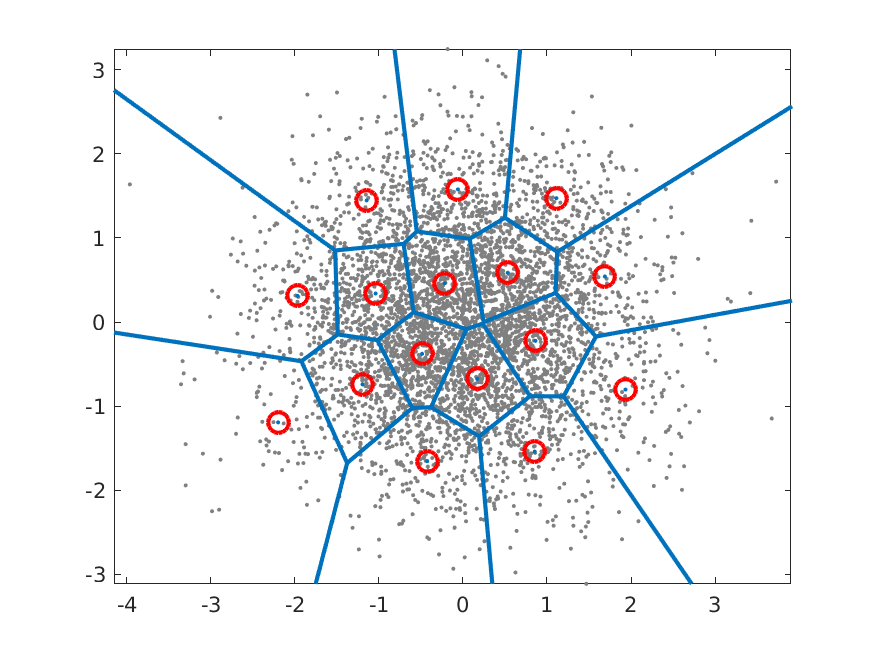
\includegraphics[scale=0.5]{images/vq_visualization.png}
    \caption{Illustration of vector quantization discrete clustering of the 2D latent space \cite{vq_visualization_website}. The grey dots are embeddings of the continous latent space, and the red dots are the code vectors from the codebook. In this case, the codebook size is 16.}
    \label{figure:vq_visualization}
\end{figure}

This technique involves the use of a codebook, which is a discrete collection of vectors of the same size as the hidden dimension. In the VQ-VAE model, after the input passes through the encoder (which results in embeddings - which are the hidden representation of the input), the embeddings are replaced by the closest vector from the codebook (by minimizing distance between vectors). This operation allows the model to learn clusters of similar embeddings, which can be used to generate new samples. The codebook is learned during training, and the embeddings are quantized to the nearest code vector in the codebook. The codebook is learned by minimizing the loss function:

\begin{equation}
    \mathcal{L}_{\text{VQ}} = || \text{sg}[z_e] - z_q ||_2^2 + \beta || \text{sg}[z_q] - z_e ||_2^2
\label{eq:vq_loss}
\end{equation}

where $z_e$ is the encoder output, $z_q$ is the quantized output, $\text{sg}[\cdot]$ is the stop gradient operation (which prevents gradients from flowing through the quantization operation), and $\beta$ is a hyperparameter that controls the weighting of the two terms in the loss function. The first term in the loss function is the quantization loss, which measures the distance between the encoder output and the quantized output. The second term is the commitment loss, which measures the distance between the quantized output and the encoder output. The commitment loss encourages the model to use the codebook, and prevents the model from ignoring the quantization operation.

\subsection*{Architecture}

ABC

\subsection*{Training}

ABC
% \newpage

% % VQ-GAN
% \section{VQ-GAN}
\label{sec:vqgan}

\begin{figure}
    \centering
    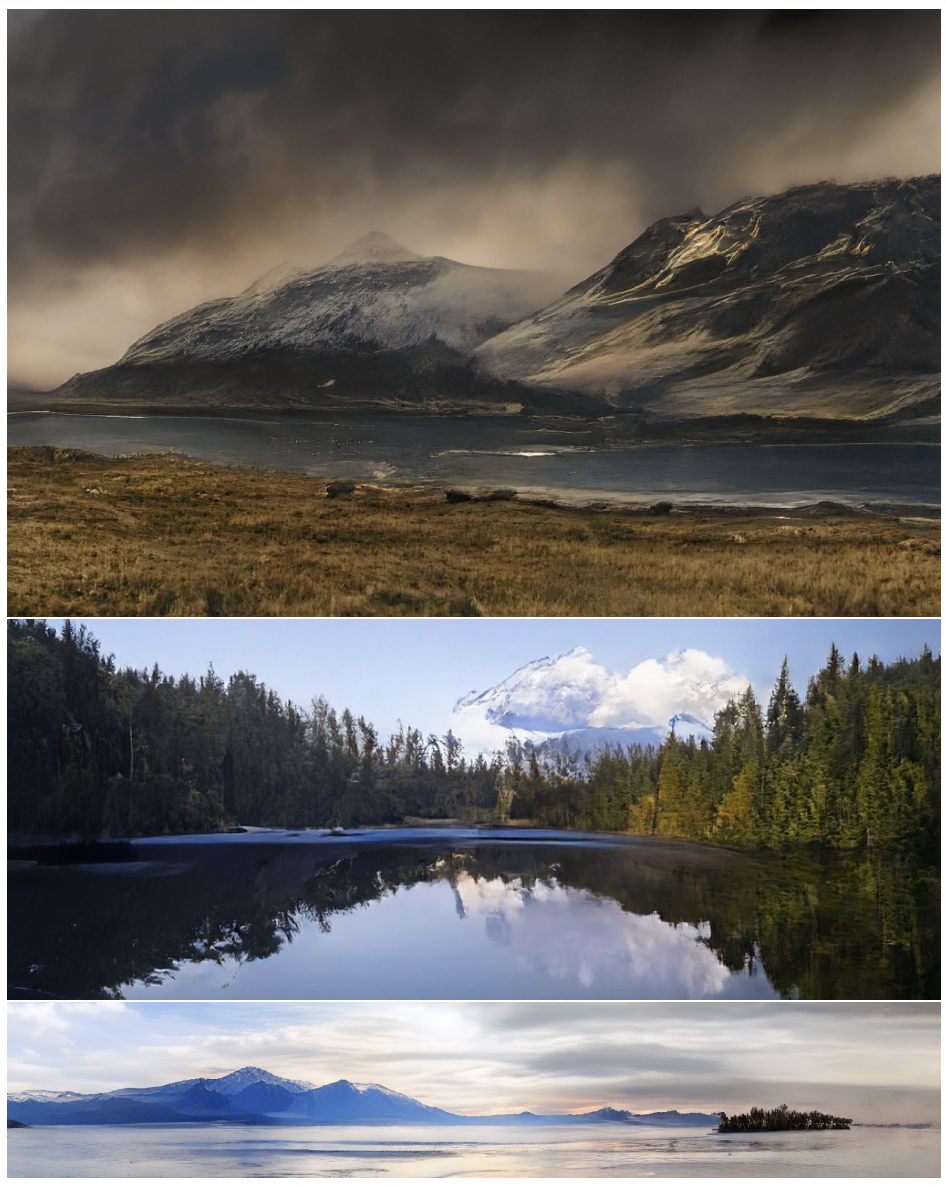
\includegraphics[width=0.5\textwidth]{images/vqgan_samples.png}
    \caption{Samples generated by VQ-GAN with different resolutions (top to bottom: 1280x832, 1024x416, 1280x240), conditioned on semantic layouts from S-FLCKR dataset.}
\end{figure}

Vector Quantized Generative Adversarial Network (VQ-GAN) \cite{vqgan} is a deep learning model capable of generating high-quality images, with the ability of conditioning (text, images, semantic masks and human pose). The architecutre of VQ-GAN is based on previous works: Vector Quantized Variational Autoencoder (VQ-VAE) \cite{vqvae} (section \ref{sec:vqvae}), transformers \cite{transformer} (appendix \ref{appendix:transformers}), and Generative Adversarial Network (GAN) \cite{gan} (section \ref{sec:gan}). The main premises of VQ-GAN is instead of representing an image with pixels, they represent it as a composition of perceptually rich image constituents from a codebook.

VQ-GAN takes the best of both worlds: the ability to generate high-quality images from GANs and the ability to condition the generation process from VQ-VAE using transformers. The combination of the expressivness of transformers and the inductive bias \footnote[1]{Inductive bias is the ability to capture local information in the image, which is why CNN is chosen,  because of the pooling layers.} of CNNs \cite{cnn} in this work showed significant improvements in image generation tasks compared to previous models. Transformers can learn long-range dependencies, whereas CNNs are better fit at learning local features and structures of images. Additional benefit in using a transformer is that is allows the model to output images of various resolutions, which is not possible with previous works.

\begin{figure}
    \centering
    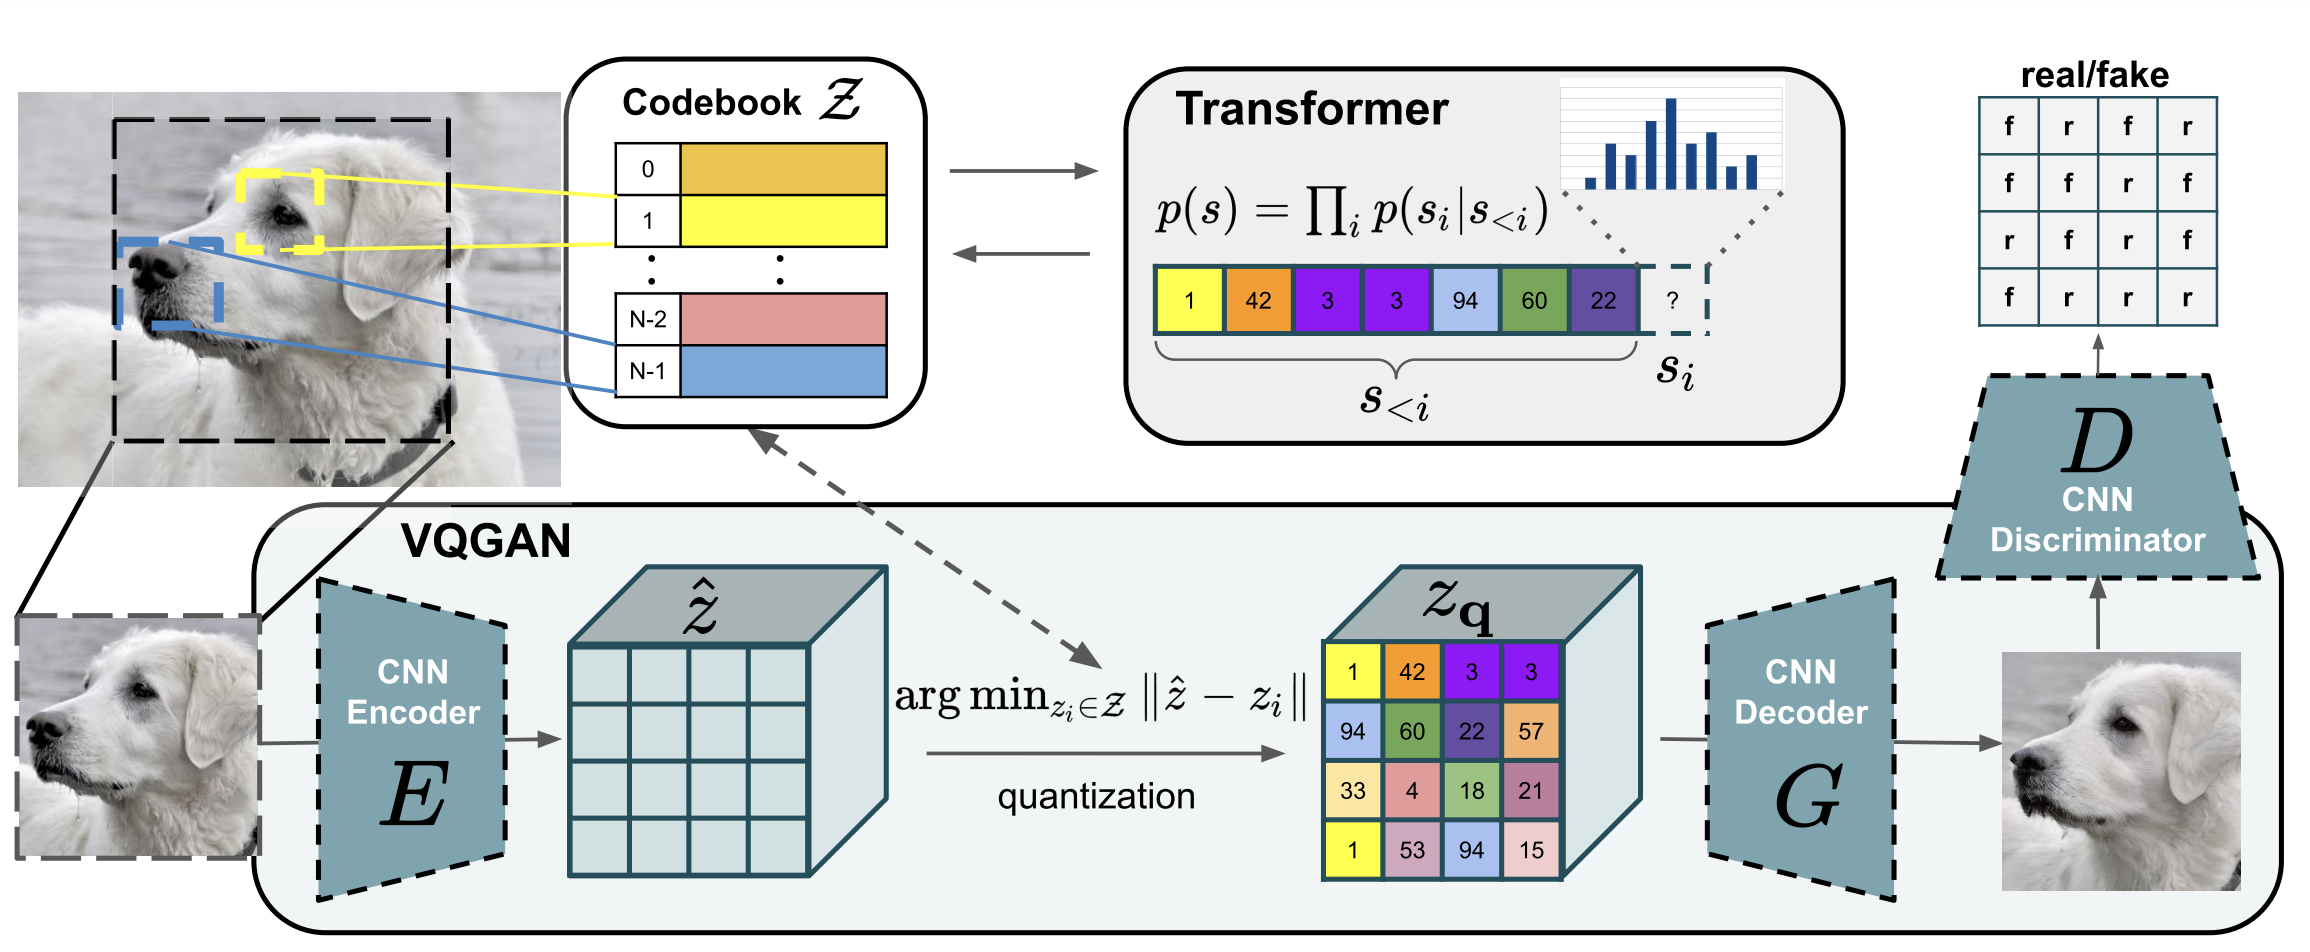
\includegraphics[width=\textwidth]{images/vqgan_architecture.png}
    \caption{VQ-GAN architecture \cite{vqgan}. The bottom rectangular part is the VQ-VAE module with the addition of a descriminator $D$ (right), and the top part is the autoregressive transformer network that predicts the next code vector $s_i$ based on previous outputs $s_{<i}$.}
    \label{fig:vqgan_architecture}
\end{figure}

In the source code of VQ-GAN the researchers used the VGG16 \cite{vgg16} architecture as the backbone of the encoder and decoder networks, but they mentioned that other architectures can be used as well, depending on the generative task. In addition, the authors used the minGPT \cite{mingpt} architecture as the transformer module (more commonly known as GPT-2, which is based on the OpenAI's model GPT-1).

The non-differential operation of quantization is a problem we saw previously in VQ-VAE (subsection \ref{subsec:vqvae_vq}), and to solve this problem the authors said that they used the straight-through estimator \cite{ste} to backpropagate the gradients through the quantization process, similarly to VQ-VAE.






\subsection{Architecture}

THe architecture of VQ-GAN is shown in figure \ref{fig:vqgan_architecture}. The training involves feeding images $x \in X$ of size $x \in \mathbb{R}^{H \times W \times 3}$ \footnote[2]{The training dataset was of size $256 \times 256 \times 3$.} to the encoder $E$ to get the latent representation $\hat{z}$ of size $\hat{z} \in \mathbb{R}^{h \times w \times n_z}$, where $n_z$ is the dimension of each codebook vector. These representation are then quantisized by the VQ module to get the discrete latent representation $z_q \in \mathbb{R}^{h \times w \times n_z}$. This operation converts latent vectors to indencies of code vectors by nearest neighbor code vector (index in the codebook points to a code vector). Using $z_q$ vectors, the CNN decoder $G$ then reconstructs the image $\hat{x}$. A discriminator $D$ is used to distinguish between real and fake (generated) pixel patches of size 16x16. This module encourages the model to generate finer details and local patterns in the image, leading to better overall quality.

The autoregressive transformer is used to predict the embeddings $z_q$ and provide the decoder $G$ the nessessary information to generate a new image, compared to PixelCNN model \cite{pixelcnn} which uses transformer for pixel-by-pixel prediction.




\subsection{Training}

The model is trained in two stages: in the first phase, the VQ module is trained to learn a discrete latent representation of the input data (learn the codebook), and the second phase trains the transformer module to predict the code vectors sequence that will be used to generate the output image.

The loss function of training the model to learn the codebook is given by: (similar to the VQ-VAE loss function in equation \ref{eq:vqvae_loss}):

\begin{equation}
    \mathcal{L}_{\text{VQ}} (E, G, \mathcal{Z}) = \Vert x - \hat{x} \Vert ^2 + \Vert \text{sg}[E(x)] - z_q \Vert ^2_2 +  \beta \Vert \text{sg}[z_q] - E(x) \Vert ^2_2
\end{equation}

where the first term is the MSE reconstruction loss (similar to equation \ref{eq:mse}), the second term is the quantization error, and the third term is the commitment loss. The reconstruction loss is intended to train the decoder $G$ to output (reconstruct latents $z_q$ to an image) images of similar distribution to the dataset. The quantization loss encourages the model to move the codebook vectors torwards the encoder outputs, so to match the encoder's output distribution (gradients are calculated for $z_q$ and not $\text{sg}[E(x)]$ because of the stop gradient operation). The commitment loss encourages the encoder to "commit" to outputting embeddings that are close to the codebook vectors.

However, instead of the MSE loss, the authors used a perceptual loss \footnote[4]{Perceptual loss measures the difference between the high-level features of two images (a generated image and an image from the dataset). Typically the high-level features are extracted by pretrained CNNs.} and \textbf{introduced an adversarial training procedure with a patch-based discriminator $D$} that tries to distinguish between real and fake pixel patches of size 16x16 of an image. The loss function of the discriminator is given by:

\begin{equation}
    \mathcal{L}_{\text{GAN}}(\{E,G,Z\}, D) = [\log D(x) + \log (1-D(\hat{x}))]
\end{equation}

If $D$ outputs 1, then the image is from the dataset (real), and if it outputs 0, then the image is fake (generated by the decoder $G$). Just like in GAN, the discreiminator objective is to maximize the probability of assigning the correct label to the input image and in the loss function the first term encourages the discriminator to output 1 because $\log D(x)$ approaches 0 when $D(x)$ approaches 1, and the second term encourages the discriminator to output 0 for fake images because $\log (1-D(\hat{x}))$ approaches 0 when $D(\hat{x})$ approaches 0.

Combining both the VQ loss and the adversarial loss, the total loss function is given by:

\begin{equation}
    \mathcal{Q^*} = \arg \min_{E, G, Z} \max_D \mathbb{E}_{x \sim p(x)} [\mathcal{L}_{\text{VQ}} + \lambda \mathcal{L}_{\text{GAN}}]
\end{equation}

The $\lambda$ hyperparameter is used to balance the contribution of adversarial loss relative to the VQ loss.

\begin{figure}
    \centering
    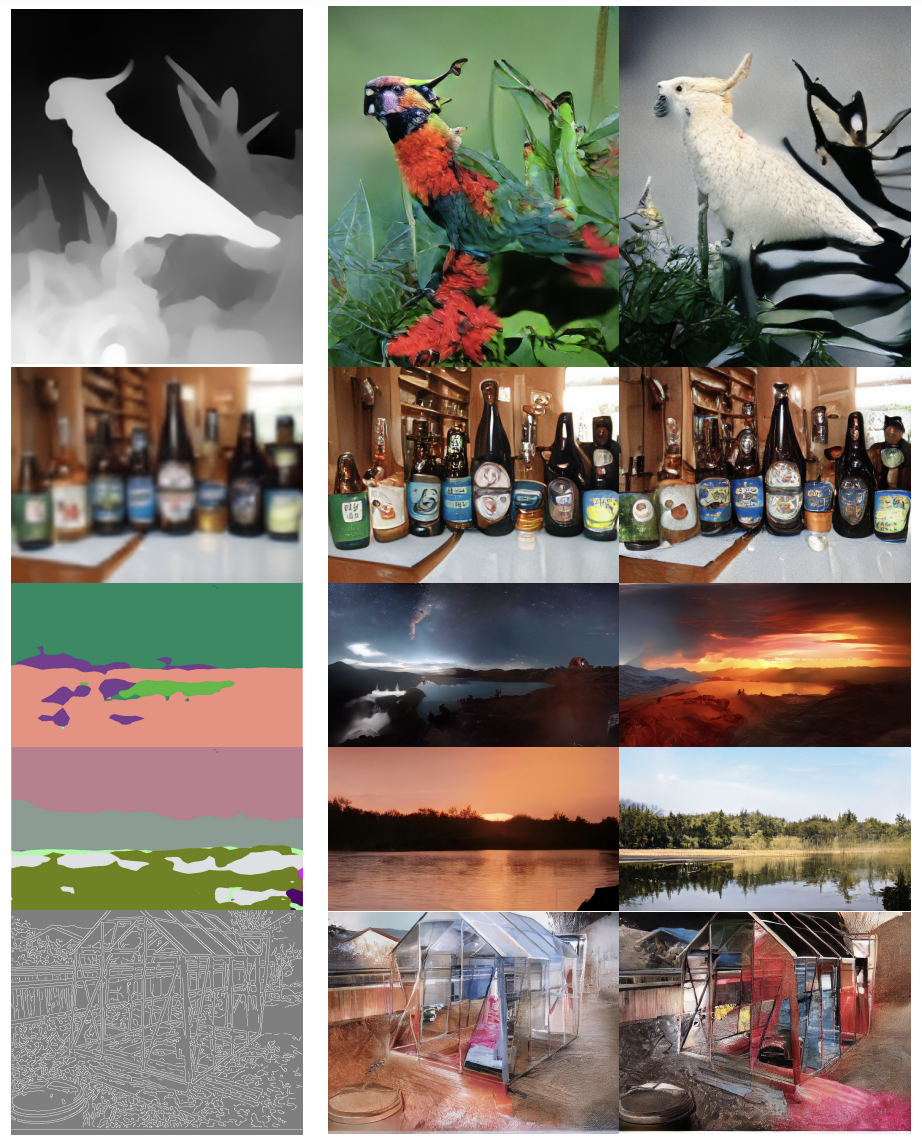
\includegraphics[width=0.5\textwidth]{images/vqgan_samples2.png}
    \caption[Caption for LOF]{Samples generated by VQ-GAN by different tasks and different resolutions. From top to bottom: depth-to-image on RIN dataset, stochastic super resolution\footnotemark on RIN dataset, 3rd and 4th row are semantic synthesis (semantic masks) on S-FLCKR dataset, and bottom row are edge synthesis on IN dataset.}
\end{figure}


\footnotetext{Super resolution is a task that generates high-resolution image from a single low-resolution image while maintaining the spatial information of the image.}

The second phase of the training involves maximizing the transformer objective. The transformer learns to predict the distribution of possible next indices, which allows us to directly maximize the log-likelihood (appendix \ref{appendix:likelihood_function}) of the data representation:

\begin{equation}
    \mathcal{L}_{\text{transformer}} = \mathbb{E}_{x \sim p(x)} [- \log p(x)]
\end{equation}

To summorize, the VQ-GAN model has 3 loss functions: the VQ loss (which trains the model to learn the codebook vectors), the adversarial loss (which trains the model to generate realistic images), and the transformer loss (which trains the model to predict the next code vector autoregressivly).







\subsection{Conditional generation}

% TODO: Finish
After the two-phase training is finished, the transformer is used to predict a sequence $s$ which is sequence of indencies to code vectors. Each token $s_i$ coresponds to an index in the codebook. So a code vector is autoregressivly predicted based on the previous tokens $s_{<i}$, which provides the nessessary embeddings $z_q$ for image synthesis ($p(s) = \prod_{i} p(s_i | s_{<i})$). If the image generation process involves a condition basis $c$, such as text, images, depth map, semantic layout or pose, then another VQ-GAN model is trained on these kind of tasks, which obtain a new codebook $Z_c$ which are the representation $r$ of $c$. Then, this representation is prepended to $s$ which restricts the computation of the negative log-likelihood to entries $p(s_i | s_{<i}, r)$. This new sequence is then given to the transformer in the first model to generate the image based on the condition $c$ (figure \ref{fig:vqgan_conditional_generation}).

\begin{figure}
    \centering
    \label{fig:vqgan_conditional_generation}
    \caption{The conditioned input sequence given to the transformer, based on the spatial condition information $c$. The middle rectangle represents a 'begin sequence' token.}
    
\begin{tikzpicture}
        \def \rectheight{0.5}

        % Draw the first rectangle
        \draw (0,0) rectangle (3,\rectheight);
        \node at (1.5,\rectheight / 2) {r};
        
        % Draw the middle rectangle
        \draw (3,0) rectangle (4,\rectheight);
        
        % Draw the third rectangle
        \draw (4,0) rectangle (7,\rectheight);
        \node at (5.5,\rectheight / 2) {s};
    \end{tikzpicture}
\end{figure}






\subsection{Sliding window technique for generating high-resolution images}

\begin{figure}[h]
    \centering
    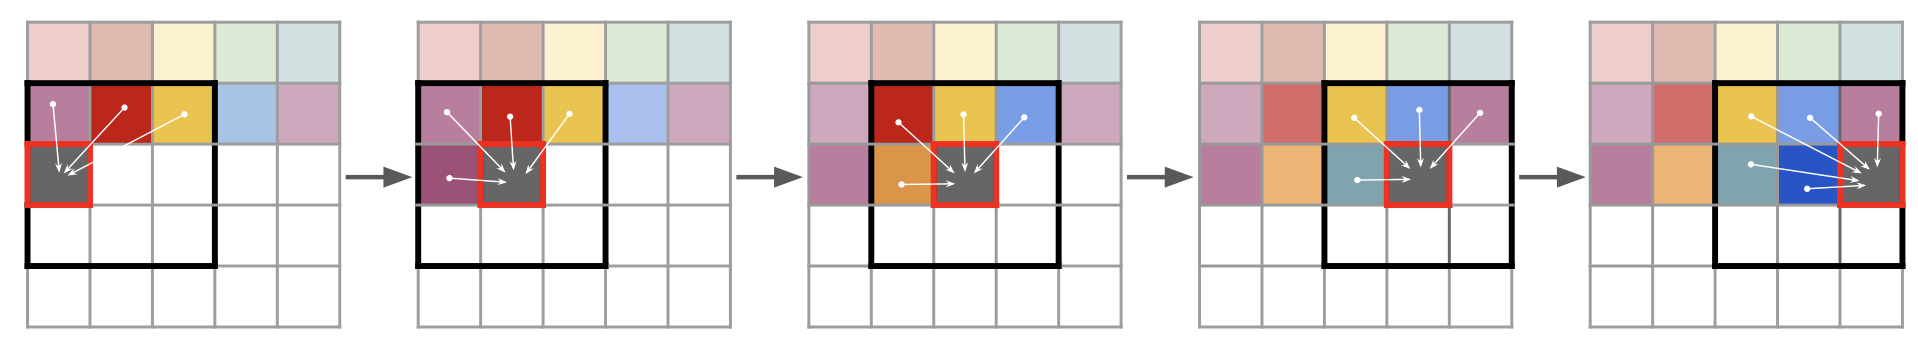
\includegraphics[width=0.75\textwidth]{images/vqgan_sliding_attention.png}
    \caption{Sliding window attention technique for generating high-resolution images. The output image is divided into patches of size 16x16=256 and by using attention mechanism, the transformer module is able to autoregressivly generate the next code vector $s_i$ based on the previous outputs $s_{<i}$ (the context).}
    \label{fig:vqgan_sliding_window}
\end{figure}

Due to the attention mechanism in transformers (quadratic computation for number of tokens, because each token requires attention to all other tokens), the model is limited in the size of the transformer sequence (in the paper they used 256 tokens). Although the encoder can reduce the dimentionality of images, the researchers noticed significant degration in generation quality. To solve this problem, they work patch-wise and crop input images to match the maximum token count in the transformer module.

To sample images, they also work patch-wise and the transformer autoregressivly predicts the next token based on the window context (figure \ref{fig:vqgan_sliding_window}).


% \newpage

% References / bibliography
\printbibliography
\newpage

% Appendix
\section{Appendix}


\subsection{Latent Variables}
\label{appendix:latent_variables}
Latent variables represent the underlying constructs that we can't directly measure. They are denoted by $z$. In the sampling process, we assume a specific probability distribution for $z$ denoted as $P(z)$. This distribution reflects prior knowledge about the latent variable. Usually its the normal distribution (Gaussian):

\[ P(z) = \mathcal{N} (\mu, \Sigma) \]

where $\mu$ is the mean, $\Sigma$ is the covariance of $z$ and $P(z)$ is called the \textbf{prior distribution}. This represents our belief about the distribution of the latent variables before considering the observed data. It helps us incorporate prior knowledge into the model.

Once the observed data ($x$) are collected, the goal is to estimate the \textbf{posterior distribution} of the latent variables, denoted by $P(z|x)$.  This distribution reflects our updated belief about the latent variables after considering the observed data.  Bayes' theorem provides the framework for obtaining the posterior distribution:

\[ P(z|x) = \frac{P(x|z) \cdot P(z)}{P(x)} \]

where $P(x|z)$ is the likelihood function, representing the conditional probability of observing $x$ given a specific value of $z$.


\begin{equation*}
  \left.\begin{aligned}
  z \sim P(z)\\
  x \sim P(x|z)
\end{aligned}\right\} P(x,z) = P(x|z) \cdot P(z)
\end{equation*}


Let's take a real-life example. We know that humans have high intelligence, but we don't have direct measurement for intelligence. IQ tests however, imperfectly measure (estimates) some part of our intelligence. We say that the observable variable is the IQ score, since we can directly and perfectly measure it, and the latent variable is the intelligence. One can describe such relationship with a simple graph:


\begin{center}
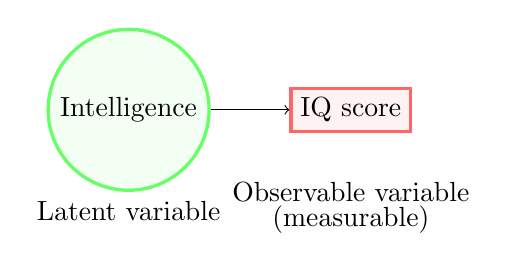
\begin{tikzpicture}[
  roundnode/.style={circle, draw=green!60, fill=green!5, very thick, minimum size=7mm},
  squarednode/.style={rectangle, draw=red!60, fill=red!5, very thick, minimum size=5mm},
]

% Nodes
\node[squarednode] (maintopic) {IQ score};
\node[roundnode] (intelligence) [left=of maintopic] {Intelligence};

% Text labels with positioning
\node [below=of intelligence, yshift=10mm] {Latent variable};
\node [below=of maintopic, yshift=5mm] {Observable variable};
\node [below=of maintopic, yshift=2mm] {(measurable)};

% Lines
\draw[->] (intelligence.east) -- (maintopic.west);

\end{tikzpicture}
\end{center}

This is why we must first measure or observe values $x$ (IQ score), so we can estimate $P(z|x)$ (intelligence). We know that the IQ score tests is Gaussian (normal) distributed with mean ($\mu$) of 100 with standard deviation ($\sigma$) of 15 points. We can say that $P(intelligence)$ is the prior distribution, because it represents our initial belief of possible values of intelligence. If we have little to no prior knowledge about intelligence, we can also assume its uniform distributed, similarly to IQ score.

The posterior distribution $P(intelligence|IQ)$ is the updated belief about the possible values of intelligence \textbf{after} we observed their IQ score. It takes into account the prior knowledge and the information from observed variables, such as IQ.


\subsection{Likelihood function}
\label{appendix:likelihood_function}

Likelihood function in the realm of generative models, is often used to capture the underlying data distribution (generate data points with similar likelihood to the training data distribution).

The formal notion of likelihood function is: $L(x | \theta)$, which reflects the probability of a specific data point ($x$) being generated by the model with its current parameters ($\theta$). We want to maximize this term: $\underset{\theta}{\arg\max}\ L(x | \theta)$. In many cases it's computationally more convenient to maximize the \textbf{log-likelihood} function instead, as the logarithm is a monotonic function (always increasing or decreasing, and therefor the log of the function is also monotonic):

\[
    \hat{\theta}_{MLE} = \underset{\theta}{\arg\max} \ \log L(\mathbf{x} | \theta)
\]

Since directly calculating the likelihood is often intractable, methods like \textbf{maximum likelihood estimation (MLE)} optimize $\theta$ indirectly. To address intractability, approaches such as \textbf{Evidence Lower Bound (ELBO)} are used as alternative loss functions. Additionally, adversarial training is widely employed in GAN-based models.

\subsection{Variational Inference (VI)}
\label{appendix:variational_inference}

Variational inference (VI) is a technique used to approximate complex posterior distributions in Bayesian inference. Instead of directly maximizing the log-likelihood function, VI aims to minimize the \textbf{Kullback-Leibler (KL) divergence} between an approximate posterior distribution and the true posterior distribution (for instance, learn the distribution of 2D points that are generated by the model, which is estimation of another distribution we want the model to learn, for instance, Gaussian). This is often achieved by minimizing a proxy loss function, such as the \textbf{Evidence Lower Bound (ELBO)}, which is tractable (can be effectively computed) to optimize. By minimizing the ELBO, VI effectively guides the approximate posterior distribution towards the true posterior distribution.
\subsection{Kullback-Leibler (KL) divergence}
\label{appendix:kl_divergence}

\begin{figure}
    \centering
    \caption{Showcase of KL-Divergence of three different normal distributions. The divergence between two normal distributions can occur in both mean and variance. Mean (or expectation) is the center of the distribution, while variance is the spread of the distribution.}
    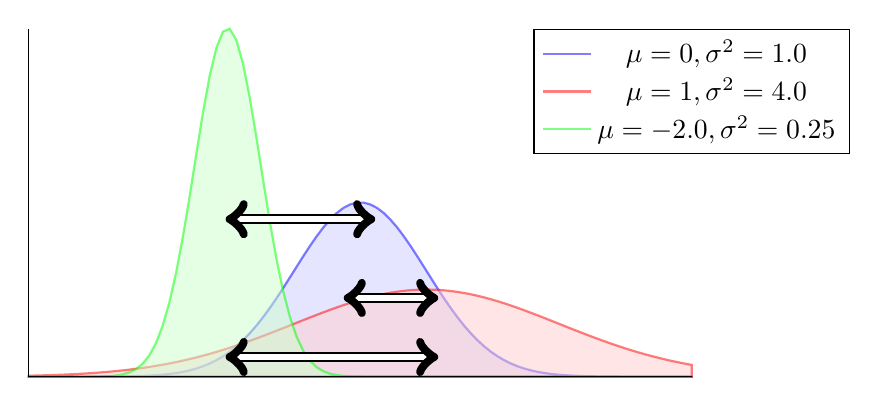
\begin{tikzpicture}
        \begin{axis} [
          no markers, 
          domain=-5:5, 
          samples=100,
          axis lines*=left, 
          height=6cm, 
          width=10cm,
          xtick=\empty, 
          ytick=\empty,
          enlargelimits=false, 
          clip=false, 
          axis on top,
          grid = major,
          legend style={at={(1,1)}, anchor=north, legend columns=1},
        ]

        % Define variables (mean, variance)
        \pgfmathsetmacro{\muA}{0}
        \pgfmathsetmacro{\sigmaA}{1}
        \pgfmathsetmacro{\varA}{\sigmaA^2}
        
        \pgfmathsetmacro{\muB}{1}
        \pgfmathsetmacro{\sigmaB}{2}
        \pgfmathsetmacro{\varB}{\sigmaB^2}
        
        \pgfmathsetmacro{\muC}{-2}
        \pgfmathsetmacro{\sigmaC}{0.5}
        \pgfmathsetmacro{\varC}{\sigmaC^2}
    
        % Blue
        \addplot[blue, thick, fill=blue!20, opacity=0.5] 
        {1/sqrt(2*pi*\sigmaA^2) * exp(-0.5 * ((x-\muA)/\sigmaA)^2)} \closedcycle;
        \addlegendentry{$\mu = \muA, \sigma^2 = \varA$};

        % Red
        \addplot[red, thick, fill=red!20, opacity=0.5] 
        {1/sqrt(2*pi*\sigmaB^2) * exp(-0.5 * ((x-\muB)/\sigmaB)^2)} \closedcycle;
        \addlegendentry{$\mu = \muB, \sigma^2 = \varB$};

        % Green
        \addplot[green, thick, fill=green!20, opacity=0.5] 
        {1/sqrt(2*pi*\sigmaC^2) * exp(-0.5 * ((x-\muC)/\sigmaC)^2)} \closedcycle;
        \addlegendentry{$\mu = \muC, \sigma^2 = \varC$};
        
        \end{axis}

        % Arrows between distributions
        % Blue, Green
        \draw[{<._[sep=-4pt]}-{_[sep=-4pt].>}, line width=0.8pt, double, double distance=2pt] (2.5,2) -- (4.4,2);
        % Green, Red
        \draw[{<._[sep=-4pt]}-{_[sep=-4pt].>}, line width=0.8pt, double, double distance=2pt] (2.5,0.25) -- (5.2,0.25);
        % Blue, Red
        \draw[{<._[sep=-4pt]}-{_[sep=-4pt].>}, line width=0.8pt, double, double distance=2pt] (4,1) -- (5.2,1);

    \end{tikzpicture}
    \label{fig:kl_divergence}
\end{figure}

Kullback-Leibler (KL) divergence allows us to measure the difference between two probability distributions, $P$ and $Q$. It essentially quantifies how much information is lost when using distribution $Q$ to approximate distribution $P$.

In various applications, we deal with situations where we have a true underlying distribution (P) representing the actual data generation process, but we might not know its exact form. We might have another distribution (Q), perhaps a model we've built, that we want to use to represent or approximate the true distribution. KL divergence helps us understand how well Q captures the information present in P. In other words, \textbf{how much diverged the distribution Q is from the distribution P}. See figure \ref{fig:kl_divergence} for a visual representation.

The mathematical formula for KL-divergence is:

\begin{equation}
\label{eq:kl-divergence}
    D_{KL}(P || Q) = \sum_{x \in X} P(x) \cdot log(\frac{P(x)}{Q(x)})
\end{equation}

where $x \in X$ represents all the possible values within the data space ($X$).

A KL-divergence value of 0 indicate that the distribution $Q$ perfectly captures the distribution $P$, and larger numbers indicate higher disparity.

KL-divergence measures information lost, so if both $P,Q$ are Gaussian distributions with the same mean and standard deviation, we have no information lost. But if the standard deviation or the mean is different, KL-divergence measures that. On the other hand, directly integrating the distributions and measuring the area under the curve (AUC) will not show information loss if the standard deviation is the same, but the mean is different.


Other notations are used as well: $p_\theta(x_i), q_\phi(x_i)$. Most of the time we are dealing with small numbers in the probabilities, which will get multiplied with other small numbers, which may result in rounding to zero. So instead we generally compute \textbf{log-likelihood}: $log\ p_\theta(x_i), log\ q_\phi(x_i)$. Now to compare two distributions we can compute the difference: $log\ p_\theta(x_i) - log\ q_\phi(x_i)$ and if that subtraction result in zero that means that our approximated distribution $q$ is identical to ground truth $p$. We can rewrite it like so: 

\begin{equation}
\label{eq:log-likelihood}
    log\ [\frac{p_\theta(x_i)}{q_\phi(x_i)}]
\end{equation}

which is also sometimes called \textbf{log-likelihood ratio}.

In reality, we are only interested in the \textbf{average difference} between $p_\theta$ and $q_\phi$. Because we are dealing with random variables $x \in X$, instead of average we say \textbf{expected value} of a random variable. Weighted average of instances of random variables is:

\begin{equation*}
    \mathbb{E}_{p_\theta} [X] = \sum_{i=1}^{\infty} x_i p_\theta(x_i)
\end{equation*}

where $x_i$ is the state of the random variable, and $p_\theta(x_i)$ is the weight (weight of contribution to the average). A more general formulation is given by:

\begin{equation*}
    \mathbb{E}_{p_\theta} [h(X)] = \sum_{i=1}^{\infty} h(x_i) p_\theta(x_i)
\end{equation*}

where $h(X), h(x_i)$ is a function of random variable $x_i \in X$. This formulation works for discrete random variable, here is the formulation for continuous random variable:

\begin{equation*}
    \mathbb{E}_{p_\theta} [h(X)] = \int_{\mathbb{R}} h(x) p_\theta(x) dx
\end{equation*}

Let's get back to the average likelihood (equation \ref{eq:log-likelihood}), we can set $h(X) = log\ [\frac{p_\theta(x_i)}{q_\phi(x_i)}]$, and we get:

\begin{equation*}
    \sum_{i=1}^{\infty} p_\theta(x_i) log\ [\frac{p_\theta(x_i)}{q_\phi(x_i)}]
\end{equation*}

where $p_\theta(x_i)$ is the weight. This equation is called the \textbf{KL-divergence}:

\begin{equation}
\label{eq:kl_divergence}
    \mathbb{E}_p [log\ \frac{p_\theta(x_i)}{q_\phi(x_i)}]
    =
    \sum_{i=1}^{\infty} p_\theta(x_i) log\ [\frac{p_\theta(x_i)}{q_\phi(x_i)}]
    =
    D_{KL} (p_\theta || q_\phi)
\end{equation}

In short, this is the expected value of the log-likelihood ratio (of discrete random variable). For continuous random variable we get similar formula:

\begin{equation}
\label{eq:kl_divergence_continous}
    \mathbb{E}_p [log\ \frac{p_\theta(x_i)}{q_\phi(x_i)}]
    =
    \int_{\mathbb{R}} p_\theta(x) log\ [\frac{p_\theta(x)}{q_\phi(x)}] dx
    =
    D_{KL} (p_\theta || q_\phi)
\end{equation}

One problem we are dealing with is the infinity space in both equations.  To get around it, we can use the \textbf{law of large numbers} which says:

\begin{equation*}
    \frac{1}{N} \sum_{i=1}^N h(x_i) \approx \mathbb{E}_p [h(X)]
\end{equation*}

and we get:

\begin{equation}
    D_{KL} (p_\theta || q_\phi) \approx
    \frac{1}{N} \sum_{i=1}^N log\ [\frac{p_\theta(x_i)}{q_\phi(x_i)}]
\end{equation}

Credit to \cite{dk-divergence-math-explanation} for the math explanation.
\subsection{Evidence Lower Bound (ELBO)}
\label{appendix:elbo}

Evidence Lower Bound (ELBO) provides an efficient way to optimize and train models that are based on variational inference (often called latent models), like VAEs or GANs. ELBO is an estimation for the log-likelihood function, and since the likelihood function is intractable in latent models (that use latent variables $z$) to calculate directly, ELBO is used instead as approximation (its tractable). ELBO achieves this by setting a lower bound on the likelihood of observing data $x$. By maximizing ELBO we essentially optimize the model by maximizing likelihood.

As we saw in equation \ref{eq:vae_posterior} the likelihood function we want to optimize is:

\begin{equation}
    p(x) = \int p(x | z) \cdot p(z) dz
\end{equation}

where $p(x)$ is the likelihood of observing data $x$, $p(x | z)$ is probability of reconstructing $x$ given latent variable $z$,  $p(z)$ is the prior distribution of latent variable $z$, and the integral is over all possible values of $z$ (if $z$ is discrete, the integral is replaced by a sum).

The reason this integral is intractable is because it is computationally expensive to calculate the likelihood of all possible values of $z$. To solve this, we can use ELBO (also defined at equation \ref{eq:vae_elbo}), which is defined as:

\begin{equation}
    \text{ELBO} = \mathbb{E}_z[\log p(x | z)] - KL(q(z) \Vert p(z))
    \label{eq:elbo}
\end{equation}

where $\mathbb{E}_z[\log p(x | z)]$ is the expected reconstruction loss, and $KL(q(z) \Vert p(z))$ is the Kullback-Leibler divergence (see appendix \ref{appendix:kl_divergence}) between the approximate posterior $q(z)$ and the prior distribution $p(z)$.

The reason this is tractable is because we use mean (expectation) instead of integrating, and both the reconstruction loss and KL divergence are well defined and tractable. 

\subsection{VQ-VAE}

In listing \ref{lst:vq_codebook} we can see that the researchers divided the code vectors by number of embeddings, which normalizes the vectors in order to stabilize the training (the codebook vectors will have unit variance).

\begin{lstlisting}[language=Python, label=lst:vq_codebook, caption=Code of the quantisizer module of VQ-VAE paper. Shows the initialization of the codebook vectors.]
    class VectorQuantizer(nn.Module):
    """
    Discretization bottleneck part of the VQ-VAE.

    Inputs:
    - n_e : number of embeddings
    - e_dim : dimension of embedding
    - beta : commitment cost used in loss term, beta * ||z_e(x)-sg[e]||^2
    """

    def __init__(self, n_e, e_dim, beta):
        super(VectorQuantizer, self).__init__()
        self.n_e = n_e
        self.e_dim = e_dim
        self.beta = beta

        self.embedding = nn.Embedding(self.n_e, self.e_dim)
        self.embedding.weight.data.uniform_(-1.0 / self.n_e, 1.0 / self.n_e)
\end{lstlisting}




\begin{lstlisting}[language=Python, label=lst:vqvae_distance, caption=Euclidean distance calculation in VQ-VAE paper between embedding and codebook vectors $\Vert z-e \Vert$.]

    def forward(self, z):
        """
        Inputs the output of the encoder network z and maps it to a discrete 
        one-hot vector that is the index of the closest embedding vector e_j

        z (continuous) -> z_q (discrete)

        z.shape = (batch, channel, height, width)

        quantization pipeline:

            1. get encoder input (B,C,H,W)
            2. flatten input to (B*H*W,C)

        """
        # reshape z -> (batch, height, width, channel) and flatten
        z = z.permute(0, 2, 3, 1).contiguous()
        z_flattened = z.view(-1, self.e_dim)
        # distances from z to embeddings e_j (z - e)^2 = z^2 + e^2 - 2 e * z

        d = torch.sum(z_flattened ** 2, dim=1, keepdim=True) + \
            torch.sum(self.embedding.weight**2, dim=1) - 2 * \
            torch.matmul(z_flattened, self.embedding.weight.t())
    
\end{lstlisting}


\begin{lstlisting}[language=Python, label=lst:vqvae_loss, caption=Loss function as defined in the VQ-VAE paper (eq. \ref{eq:vq_loss}). The detach keyword is the stop gradient operation.]
    # compute loss for embedding
    loss = torch.mean((z_q.detach()-z)**2) + self.beta * \
        torch.mean((z_q - z.detach()) ** 2)
\end{lstlisting}



\begin{lstlisting}[language=Python, label=lst:vqvae_stop_gradients, caption=Allow gradients to flow through the snapping operation.]
    # preserve gradients
    z_q = z + (z_q - z).detach()
\end{lstlisting}
\subsection{Transformers}
\label{appendix:transformers}

...

\end{document}